\documentclass[10pt]{beamer}
%%
\usepackage{pgfpages}
\usepackage{graphicx}
\usepackage{ulem}
\usepackage{color}
\usepackage{fancyvrb}
% get rid of junk
\usetheme{default}
\beamertemplatenavigationsymbolsempty
\hypersetup{pdfpagemode=UseNone} % don't show bookmarks on initial view
% font
\usefonttheme{professionalfonts}
\usefonttheme{serif}
% page number
\setbeamertemplate{footline}{%
  \raisebox{5pt}{\makebox[\paperwidth]{\hfill\makebox[20pt]{\color{gray}
        \scriptsize\insertframenumber}}}\hspace*{5pt}}
% add a bit of space at the top of the notes page
\addtobeamertemplate{note page}{\setlength{\parskip}{12pt}}

\setbeamertemplate{blocks}[rounded][shadow=true]

\AtBeginSection{
  \begin{frame}
    \begin{center}
      \structure{\Large \insertsection}
    \end{center}
  \end{frame}
}

\newcommand{\df}{{\it data.frame} }
\newcommand{\gr}{{\it GRanges} }
\newcommand{\dfs}{{\it data.frames} }
\newcommand{\mat}{{\it matrix} }

\title{HGSS Workshop : R, data manipulation, visualization, genomic ranges}
\author{Jean Monlong}
\institute{Human Genetics department}
\date{May 8th, 2015}

\begin{document}



%%%%%%%%%%%%%%%%%%%%
%% Title Slide
\begin{frame}
  \centering
  \titlepage
  \begin{minipage}{.4\textwidth}
    
\includegraphics[width=.8\linewidth]{../imgs/hgssLogo-black.png}
  \end{minipage}
  \hspace{.1\textwidth}
  \begin{minipage}{.4\textwidth}
    
\includegraphics[width=\linewidth]{../imgs/McGill-Logo1.png}
  \end{minipage}

\end{frame}

\begin{frame}{Today's topic}
  \begin{block}{}
    \begin{itemize}
    \item Advanced manipulation of \dfs.
    \item Advanced visualization.
    \item Analyzing large data.
    \end{itemize}
  \end{block}
  \begin{block}{Doodle}
    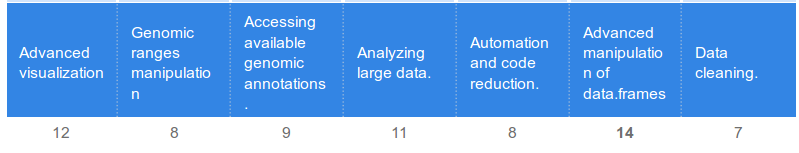
\includegraphics[width=\textwidth]{doodle-ws2.png}    
  \end{block}

  \begin{block}{Let's get started !}
    \begin{enumerate}
    \item Open R/Rstudio or whatever you use.
    \item Prepare a folder for the workshop and set it as working directory.
    \item Download {\sf dataWS2.RData} from \href{https://drive.google.com/open?id=0BwSxlHpMjRKtbUpqUGZOVkFFLUE}{\uline{there}}
    \end{enumerate}
  \end{block}
  
\end{frame}

\begin{frame}[fragile, shrink=10]{Today's packages}
  \begin{alertblock}{Installation}
    \begin{itemize}
    \item Using \verb!install.packages! for CRAN packages.
    \item Using \verb!biocLite! for Bioconductor packages.
    \end{itemize}
  \end{alertblock}
  \begin{exampleblock}{Run this}
\begin{verbatim}
install.packages(c("data.table","dplyr","ggplot2","reshape"))
source("http://bioconductor.org/biocLite.R")
biocLite(c("GenomicRanges","AnnotationHub"))
\end{verbatim}
  \end{exampleblock}
\end{frame}

\section{Large \mat}
%%
%%%    Row by row analysis
%%

\begin{frame}[fragile]{Large \mat and row-by-row analysis}
  \begin{alertblock}{Don't do this !}
    Concatenate iteratively on big data.

\begin{verbatim}
myMatrix = NULL
for(i in 1:100000){
... Instructions on myOtherMatrix[i,]
myMatrix = rbind(myMatrix, myNewLine)
}
\end{verbatim}  
  \end{alertblock}
  \begin{exampleblock}{Instead do this}
    Create the data and then fill it.

\begin{verbatim}
myMatrix = matrix(NA,100000,100)
for(i in 1:100000){
... Instructions on myOtherMatrix[i,]
myMatrix[i,] = myNewLine
}
\end{verbatim}  
  \end{exampleblock}
\end{frame}

\begin{frame}[fragile, shrink=10]{Large \mat and row-by-row analysis}

  \begin{alertblock}{Don't do this !}
    Create the data and then fill it.
    
\begin{verbatim}
myMatrix = matrix(NA,100000,100)
for(i in 1:100000){
... Instructions on myOtherMatrix[i,]
myMatrix[i,] = myNewLine
}
\end{verbatim}  
  \end{alertblock}
  \begin{exampleblock}{Instead do this}
    Use {\sf apply} and a function.
    
\begin{verbatim}
myMatrix = apply(myOtherMatrix, 1, function(myOtherMatrix.row){
   ... Instructions on myOtherMatrix.row
   return(myNewLine)
})
\end{verbatim}  
  \end{exampleblock}
\end{frame}


\section{\df}
%%
%%%   Introducing data.frames
%%

\begin{frame}[fragile, shrink=19]{\dfs}
  \begin{block}{}
    \begin{itemize}
    \item Mix between \mat and {\it list}
    \item Array form.
    \item Columns can have different data types.
    \end{itemize}
  \end{block}
  \begin{columns}
    \begin{column}{.5\textwidth}
      \begin{block}{\mat}
\begin{Verbatim}[commandchars=\\\{\}]
      samp1 samp2 samp3
gene1  \color{blue}-1.3  -1.8  -4.1\color{black}
gene2  \color{blue}-1.5  -1.2   4.9\color{black}
\end{Verbatim}
      \end{block}
    \end{column}
    \begin{column}{.5\textwidth}
      \begin{block}{\df}
\begin{Verbatim}[commandchars=\\\{\}]
 gene sample expression
\color{red}gene1  samp1       \color{blue}-1.3\color{black}
\color{red}gene2  samp1       \color{blue}-1.5\color{black}
\color{red}gene1  samp2       \color{blue}-1.8\color{black}
\color{red}gene2  samp2       \color{blue}-1.2\color{black}
\color{red}gene1  samp3       \color{blue}-4.1\color{black}
\color{red}gene2  samp3       \color{blue} 4.9\color{black}
\end{Verbatim}
      \end{block}
    \end{column}
  \end{columns}
  \begin{block}{Pros/Cons}
    \begin{columns}
      \begin{column}{.5\textwidth}
        \begin{description}
        \item[+] Dense representation of large data.
        \item[-] Accepts only one data type.
        \item[-] \underline{manual} combination with other information often required.
        \end{description}
      \end{column}
      \begin{column}{.5\textwidth}
        \begin{description}
        \item[+] Flexible.
        \item[+] Accepts several data types.
        \item[+] Can represent all the data needed for an analysis.
        \item[-] Takes more space/memory due to repetitions.
        \end{description}
      \end{column}
    \end{columns}
  \end{block}
\end{frame}

\begin{frame}[fragile,shrink=15]{\df basics}
  \begin{exampleblock}{Create a \df}
\begin{verbatim}
myDF = data.frame(gene=c("A","B","C"),id=1:3)
myDF = data.frame(gene=c("A","B","C"),id=1:3, 
                            stringsAsFactors=FALSE)
\end{verbatim}
Add parameter \verb!stringsAsFactors=FALSE}! to avoid annoying type conversion.
  \end{exampleblock}
  \begin{alertblock}{Exercise}
    Try both commands and observe the difference using \verb!str! function.
  \end{alertblock}
  \begin{exampleblock}{Access columns}
    Use $\$$ symbol for comfort and readability.
\begin{verbatim}
myDF[,1]
myDF[,"gene"]
myDF$gene
\end{verbatim}
  \end{exampleblock}
  \begin{block}{Same functions as \mat}
    {\sf colnames}, {\sf dim}, {\sf head}, {\sf str}, {\sf rbind}.
  \end{block}
\end{frame}

\begin{frame}[fragile]{Transform a \mat into a \df}
  \begin{block}{Package {\sf reshape}}
    {\sf melt} function melts a \mat into a \df using the rows and columns names.    
  \end{block}
  \begin{columns}
    \begin{column}{.5\textwidth}
      \begin{exampleblock}{Example}
\begin{verbatim}
> library(reshape)
> mat
     col1 col2 col3
row1    1    3    5
row2    2    4    6
> melt(mat)
    X1   X2 value
1 row1 col1     1
2 row2 col1     2
3 row1 col2     3
4 row2 col2     4
5 row1 col3     5
6 row2 col3     6
\end{verbatim}
      \end{exampleblock}
    \end{column}
    \begin{column}{.5\textwidth}
      \begin{alertblock}{Exercise}
        \begin{itemize}
        \item Load {\sf dataWS2.RData} and have a look at {\sf mat.ge} \mat.
        \item Create a new matrix with only the first 10 rows of {\sf mat.ge}.
        \item Create a \df from this new matrix.
        \item Add relevant column names.
        \end{itemize}
      \end{alertblock}
    \end{column}
  \end{columns}
\end{frame}

\begin{frame}[fragile,shrink=5]{Merge two \dfs}
  \begin{block}{}
    {\sf merge} function merges \dfs using their {\bf common columns}.
  \end{block}
  \begin{exampleblock}{Example}
\begin{verbatim}
df12 = merge(df1, df2)
\end{verbatim}
  \end{exampleblock}
  \begin{block}{Example - Two \dfs merged}
    \begin{columns}
      \begin{column}{.3\textwidth}
        \centering
        \resizebox{\linewidth}{!}{\begin{tabular}{|ccc|}
          \hline
          colA & colB & colC \\ \hline
          2 & 43 & france \\
          4 & 87 & france \\
          1 & 100 & spain \\ \hline
        \end{tabular}}
        \bigskip
        \resizebox{\linewidth}{!}{\begin{tabular}{|ccc|}
            \hline
            colA & colD & colE \\ \hline
            2 & TRUE & bonjour \\
            1 & FALSE & hola \\ \hline
        \end{tabular}}
      \end{column}
      \begin{column}{.6\textwidth}
        \centering
        \resizebox{\linewidth}{!}{\begin{tabular}{|ccccc|}
            \hline
            colA & colB & colC  & colD & colE\\ \hline
            2 & 43 & france & TRUE & bonjour \\
            1 & 100 & spain  & FALSE & hola\\\hline
        \end{tabular}    }
      \end{column}
    \end{columns}
  \end{block}
  \begin{alertblock}{Exercise}
    \begin{itemize}
    \item Have a look at {\sf metadata.df} \df.
    \item Update the expression \df (created previously) by merging {\sf metadata.df} information.
    \end{itemize}
  \end{alertblock}
\end{frame}

\begin{frame}[fragile]{Subset a \df}
  \begin{block}{}
    {\sf subset} function retrieves a subset of a \dfs using a condition on column names.
  \end{block}
  \begin{exampleblock}{Example}
\begin{verbatim}
coldMontreal = weatherDF[which(weatherDF$city=="Montreal" 
                            & weatherDF$celsius < -30),]

coldMontreal = subset(weatherDF, city=="Montreal" 
                                       & celsius < -30)
\end{verbatim}
  \end{exampleblock}
  \begin{alertblock}{Exercise}
    \begin{itemize}
    \item Create a \df with expression of male samples only.
    \item Create a \df with expression of the first gene.      
    \end{itemize}
  \end{alertblock}
\end{frame}




\section{Visualization with {\sf ggplot2}}
%%
%%%   GGPLOT2 concept
%%


\begin{frame}{{\sf ggplot2} package}
  \begin{block}{Introduction}
    A package to construct pretty and/or complex graphs. Many aspects of the graph are arranged automatically but everything can be specified. Easy layers addition.
  \end{block}
  
  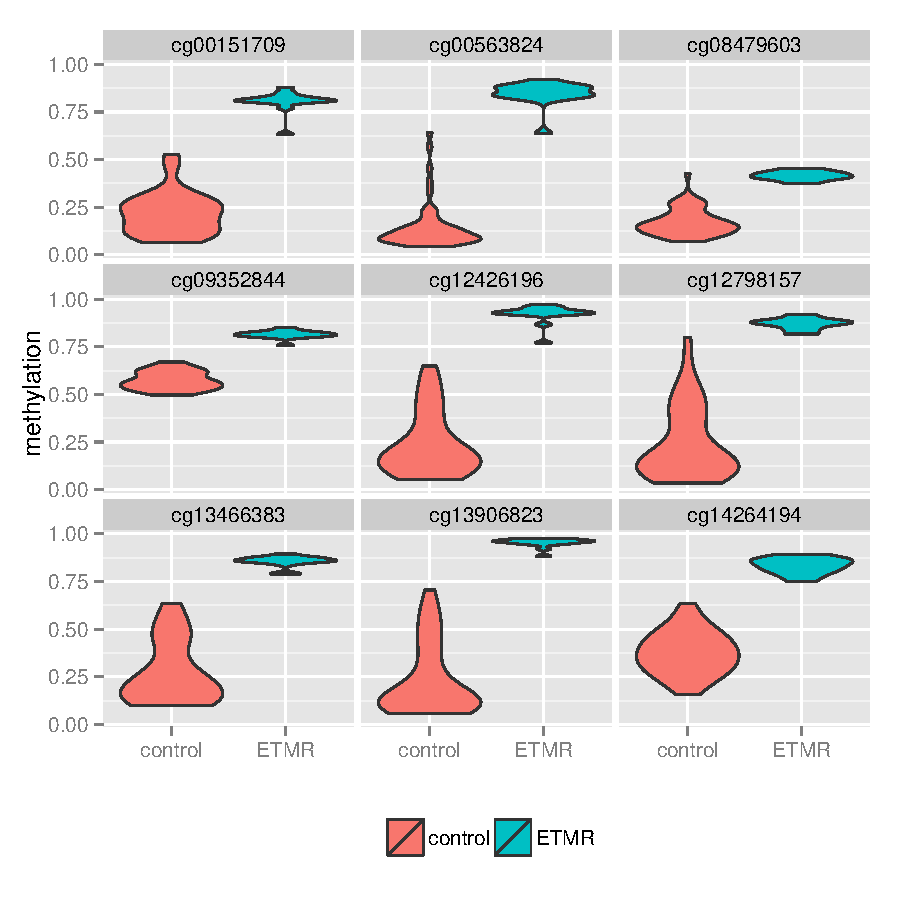
\includegraphics[height=.6\textheight]{../imgs/example-ggplot2.pdf}
  \includegraphics[height=.6\textheight,page=2]{../imgs/example-ggplot2.pdf}

\end{frame}

\begin{frame}[fragile, shrink=10]{{\sf ggplot2}}
  \begin{block}{Input : \df}
    \begin{itemize}
    \item Each row represents one {\it "observation"}.
    \item Columns represent the different information about the {\it "observations"}.
    \end{itemize}
  \end{block}

  \begin{block}{Concept}
    \begin{itemize}
    \item Start with a \verb!ggplot(...)! part and the input \df.
    \item \verb!aes(...)! defines how to use the input \df columns.
    \item Add layers : \verb!geom_*(...)!, \verb!scale_*(...)!, ...
    \end{itemize}
  \end{block}
  
  \begin{exampleblock}{Example}
\begin{Verbatim}[commandchars=\\\{\}]
library(ggplot2)
\color{blue}ggplot(\color{red}myDf\color{black}\color{blue}, aes(\color{black}x=\color{red}colA\color{black}, y=\color{red}colB\color{black}, colour=\color{red}colC\color{black}, linetype=\color{red}colD\color{black}\color{blue})) 
   + geom_point() + geom_line() + scale_y_log10()
\end{Verbatim}
  \end{exampleblock}
  
  \begin{block}{Useful online resources}
    \begin{itemize}
    \item \url{http://docs.ggplot2.org/current/}
    \item \url{http://www.cookbook-r.com/Graphs/}
    \end{itemize}
  \end{block}
  
\end{frame}

\begin{frame}[fragile, shrink=5]{Histogram}
  \begin{block}{To represent distribution of continuous values}
    \begin{itemize}
    \item \verb!geom_histogram! function.
    \item \verb!x=! to define the x-coordinate.
      \bigskip
    \item \verb!fill=! to define the bar color.
    \item \verb!position="dodge"! to put different bars side-by-side.
    \end{itemize}
  \end{block}
  \begin{exampleblock}{Example}
\begin{verbatim}
ggplot(myDF,aes(x=colA, fill=colB)) + geom_histogram()

ggplot(myDF,aes(x=colA)) + geom_histogram(fill="red")

ggplot(myDF,aes(x=colA, fill=colB)) + 
                      geom_histogram(position="dodge")
\end{verbatim}
  \end{exampleblock}
  \begin{alertblock}{Exercise}
    \begin{itemize}
    \item Plot the distribution of the expression of all genes and all samples
    \item Same but coloring the bars by genes.
    \end{itemize}
  \end{alertblock}
\end{frame}

\begin{frame}[fragile]{General functions}
  \begin{block}{}
    \begin{description}
    \item[xlab/ylab] change x/y axis label.
    \item[xlim/ylim] change x/y axis limits (range).
    \item[ggtitle] adds a title.
    \end{description}
  \end{block}
  \begin{exampleblock}{Example}
\begin{verbatim}
ggplot(myDF,aes(x=colA, fill=colB)) + geom_histogram() +
                                    xlab("column A") + 
                                    ylab("column B") +   
                                    ylim(0,10) +   
                                    xlim(1,5) +   
                                    ggtitle("An example")
\end{verbatim}
  \end{exampleblock}
  \begin{alertblock}{Exercise}
    Add relevant axis labels and title
  \end{alertblock}
\end{frame}


\begin{frame}[fragile]{Themes}
  \begin{block}{}
    \begin{itemize}
    \item \verb!theme_bw()! or \verb!theme_minimal()! for lighter graphs.
    \item \verb!theme(...)! to change specific aspects.
      \begin{itemize}
      \item \verb!legend.position="bottom"!.
      \end{itemize}
    \end{itemize}
  \end{block}
  \begin{exampleblock}{Example}
\begin{verbatim}
ggplot(myDF,aes(x=colA,y=colB,colour=colC)) + 
                    geom_point() + 
                    theme_bw() + 
                    theme(legend.position="bottom")
\end{verbatim}
  \end{exampleblock}
  \begin{alertblock}{Exercise}
    Try these on the previous graphs.
  \end{alertblock}
\end{frame}


\begin{frame}[fragile, shrink=10]{Faceting : multi-panel graphs}
  \begin{block}{}
    \begin{itemize}
    \item \verb!facet_wrap! function.
      \begin{itemize}
      \item A formula \verb!~colName! to define the column to use.
      \item \verb!ncol=! to define a number of facet columns.
      \end{itemize}
      \bigskip
    \item \verb!facet_grid! function.
      \begin{itemize}
      \item A formula \verb!colName1~colName2! to define the columns to use as facet row/column.
      \end{itemize}
      \bigskip
    \item \verb!scales="free"! to allow different axis scales.
    \end{itemize}
  \end{block}
  \begin{exampleblock}{Example}
\begin{verbatim}
ggplot(myDF,aes(x=colA)) + geom_histogram() + 
                           facet_wrap(~colB, ncol=3)

ggplot(myDF,aes(x=colA)) + geom_histogram() + 
                           facet_grid(colB~colC)
\end{verbatim}
  \end{exampleblock}
  \begin{alertblock}{Exercise}
    Show separate histograms for each gene using \verb!facet_wrap!.
  \end{alertblock}
\end{frame}


%%
%%%   Reading a large file in R
%%

\begin{frame}{Exploring Gencode annotation}
  \begin{alertblock}{Get the data}
    \begin{enumerate}
    \item Download \url{ftp://ftp.sanger.ac.uk/pub/gencode/Gencode_human/release_22/gencode.v22.annotation.gtf.gz}.
    \item Unzip it in your working directory.
    \end{enumerate}
  \end{alertblock}
  \begin{block}{Gencode file}
    \begin{itemize}
    \item Human gene reference annotation.
    \item Genes, exons, transcipts, ...
    \item More than 2 million lines.
    \item GTF format (see \url{http://www.ensembl.org/info/website/upload/gff.html}).
    \end{itemize}
  \end{block}
\end{frame}

\begin{frame}[fragile]{Basic functions}
  \begin{block}{Extra parameters in {\sf read.table}}
    \begin{description}
    \item[colClasses] a {\sf vector} with the data type of each column: e.g. {\it ``character''}, {\it ``numeric''}. Put \verb!"NULL"! to skip a column.
    \item[nrows] the number of rows to read.}
    \end{description}
  \end{block}
  \begin{block}{Read a file line by line (or by chunk)}
\begin{verbatim}
con = file(file.name)
while(length(line = readLines(con,n=1))>0){
... Instructions
}
\end{verbatim}      
  \end{block}
  \begin{block}{To test the performance}
\begin{verbatim}
system.time({
... Instructions
})
\end{verbatim}  
  \end{block}
\end{frame}

\begin{frame}[fragile]{{\sf data.table} package and {\sf fread}}
  \begin{block}{{\sf fread} function}
    \begin{description}
    \item[+] Very fast.
    \item[+] Almost no additional parameters.
    \item[-] Cannot read compressed file.
    \item[-] Has its specific format ({\it data.table})...
    \item[+] ... which can be converted into \df.
    \item[+] Very fast.
    \end{description}
  \end{block}
  \begin{exampleblock}{Example}
\begin{verbatim}
myDT = fread("myFile.tsv")
myDF = as.data.frame(myDT)
\end{verbatim}
  \end{exampleblock}
  \begin{block}{Useful parameters}
    \begin{description}
    \item[skip=] the number of lines to skip before starting to read.
    \item[select=] a {\it vector} with the columns to read.
    \end{description}
  \end{block}
\end{frame}

\begin{frame}{Exercise}
  \begin{enumerate}
  \item Use {\sf read.table} to read a few rows of {\sf gencode.v22.annotation.gtf}.
  \item Try reading the entire file (or say $500 000$ rows) using {\sf read.table}.
  \item Compare with {\sf fread} (skipping the first 5 rows).
    \bigskip
    \bigskip
  \item Use {\sf fread} to read columns $\{1,3,4,5,9\}$ of the entire file.
  \item Convert the output into a \df.
  \item Add relevant column names (see GTF format in previous slides).
    \bigskip
  \item How many elements of each feature are there.
  \end{enumerate}
\end{frame}

\begin{frame}[fragile,shrink=15]{Bar plots}
  \begin{block}{For a summary of categorical values}
    \begin{itemize}
    \item \verb!geom_bar! function.
    \item \verb!x=! to define the x-coordinate.
      \bigskip
    \item \verb!fill=! to define the bar color.
    \item \verb!position="dodge"! to put different bars side-by-side.
      \bigskip
    \item \verb!y=! to define the y-coordinate. If not defined, the number of observations is shown.
    \item \verb!stat="identity"! if the y-coordinate is defined.
    \end{itemize}
  \end{block}
  \begin{exampleblock}{Example}
\begin{verbatim}
ggplot(myDF,aes(x=colB)) + geom_bar()
ggplot(myDF,aes(x=colB)) + geom_bar(position="dodge")

ggplot(myDF,aes(x=colB,y=colC)) + geom_bar(stat="identity")
\end{verbatim}
  \end{exampleblock}
  \begin{alertblock}{Exercise}
    \begin{itemize}
    \item Create a bar plot of the number of elements in each feature.
    \item Create a bar plot of the number of elements in each chromosome.
    \item Same but coloring by feature. Try the {\it dodge} positioning.
    \end{itemize}
  \end{alertblock}
\end{frame}



%%
%%%    dplyr concept
%%
\section{\df manipulation with {\sf dplyr}}

\begin{frame}{{\sf dplyr} package}
  \begin{block}{``A Grammar of Data Manipulation''}
    {\sf dplyr} provides functions which can be combined for data manipulation.
    \begin{description}
    \item[mutate] add a new column using others.
    \item[filter] filter rows (similar as {\sf subset} function).
    \item[select] select specific columns only.
    \item[arrange] order rows using specific columns.
    \item[group\_by] groups rows according to specific columns.
    \item[summarize] summarizes each group of rows.
    \item[do] applies a function to a group of rows.
    \end{description}
  \end{block}
  \begin{block}{}
    \begin{description}
      \item[+] Works with pipes.
      \item[+] Fast.
      \item[-] Has its own format {\it tbl\_df}...
      \item[+] ... which is almost the same as \df.
    \end{description}
  \end{block}
\end{frame}

\begin{frame}[fragile]{Pipes are cool !}
  \begin{block}{}
    \begin{itemize}
    \item Pipe functions instead of embedding them.
    \item More readable.
    \item Easier to combine several functions.
    \item Avoid temporary objects.
    \item Pipe argument \verb!%>%!.
    \end{itemize}
  \end{block}
  \begin{exampleblock}{Example}
\begin{Verbatim}[commandchars=\\\{\}]
head(sort(round(sqrt(myVec))))
myVec \color{blue}%>%\color{black} sqrt \color{blue}%>%\color{black} round \color{blue}%>%\color{black} sort \color{blue}%>%\color{black} head

head(\color{blue}sort(\color{red}round(\color{black}sqrt(myVec)\color{red},digits=3)\color{blue},decreasing=TRUE)\color{black},10)
myVec \color{blue}%>%\color{black} sqrt \color{blue}%>%\color{black} round(digits=3) \color{blue}%>%\color{black} 
                        sort(decreasing=TRUE) \color{blue}%>%\color{black} head(10)
\end{Verbatim}
  \end{exampleblock}
\end{frame}

\begin{frame}[fragile, shrink=10]{{\sf dplyr} piping}
  \begin{exampleblock}{Example}
\begin{Verbatim}[commandchars=\\\{\}]
\color{blue}newDF\color{black} = \color{blue}myDF\color{black} %>% filter(\color{blue}colA\color{black} < 1) %>% 
             mutate(\color{red}colAB\color{black}=\color{blue}colA*colB\color{black}) %>% arrange(\color{blue}colAB\color{black})
\end{Verbatim}
  \end{exampleblock}
  \begin{alertblock}{Exercise}
    \begin{itemize}
    \item Create the following {\sf getAtt} function.
    \item Try this function on a few of the {\it attribute} column values.
    \item Try changing the second argument. E.g. to {\it gene\_type}.
    \item Create new columns for {\it gene\_id} and {\it gene\_type}, using {\sf mutate}.
    \item Create a bar plot of the number of {\bf genes} for each {\it gene\_type}. Try adding \verb!+coord_flip()! to the \verb!ggplot! command.
    \end{itemize}
  \end{alertblock}
  \begin{block}{{\sf getAtt} function}
    \begin{itemize}
    \item Parse a character to retrieve a value formatted as \verb!gene_id ="value"!.
    \item E.g. retrieving \color{red}\verb!ENSG111! \color{black} from \color{blue}\verb!XXX; gene_id ="ENSG111"; XXX!.
    \end{itemize}

\begin{verbatim}
getAtt <- function(attributes, att.name="gene_id"){
  sub(paste0(".*",att.name," \"([^\"]+)\";.*"), "\\1", attributes)
}  
\end{verbatim}    
  \end{block}
\end{frame}

\begin{frame}[fragile]{Exercise - Other questions}
  \begin{itemize}
  \item Find the 10 longest pseudogenes. {\tiny Hint: arrange, desc, filter.}
  \item Find the 10 shortest exons in protein-coding genes.
    \bigskip
  \item Show the distribution of gene size colored by gene type.
  \item Add \verb!scale_x_log10()! for logarithmic scale.
    \bigskip
  \item Same but using density curve : replace \verb!geom_histogram! by \verb!geom_density!.
  \end{itemize}
\end{frame}

\begin{frame}[fragile]{Grouping rows}
  \begin{block}{Operation by block}
    \begin{itemize}
    \item Using \verb!group_by()! function.
    \item Further operations are applied separately per group of rows.
    \end{itemize}
  \end{block}
  \begin{exampleblock}{Example}
\begin{verbatim}
myDF %>% group_by(colA) %>% summarize(colB.mean=mean(colB))

myDF %>% group_by(colA, colB) %>% summarize(nbAB=n())

myDF %>% group_by(colAB) %>% summarize(nbAB=n()) %>% 
                 ungroup %>% arrange(desc(nbAB)) %>% head
\end{verbatim}
  \end{exampleblock}
  \begin{block}{Tips}
    \begin{itemize}
    \item \verb!n()! gives the number of rows in the group.
    \item \verb!ungroup! removes groups.
    \item \verb!desc()! means descending order (in \verb!arrange()!).
    \end{itemize}
  \end{block}
\end{frame}

\begin{frame}[fragile]{Exercise}
  \begin{enumerate}
  \item Get the number of genes for each gene type...
  \item ... ordered by descending number of genes.
  \item Keep only genes in the 6 most common gene types OR label the rest as \verb!"others"!.
  \item Plot the new version of the gene size distribution.
    \bigskip
  \item Compute the number of exons per gene.
  \item Plot the distribution.
  \item Same zooming in the range $[0,100]$.
  \item Same coloring by gene type.
  \item Which genes have the more exons.
  \end{enumerate}
\end{frame}

\begin{frame}[fragile]{Scatterplots}
  \begin{block}{}
    \begin{itemize}
    \item \verb!geom_point! function.
    \item \verb!x=! to define the x-coordinate.
    \item \verb!y=! to define the y-coordinate.
      \bigskip
    \item \verb!colour=! to define the point color.
    \item \verb!alpha=! to define the point opaqueness.
    \item \verb!shape=!, \verb!size=! to define the point shape/size.
    \end{itemize}
  \end{block}
  \begin{exampleblock}{Example}
\begin{verbatim}
ggplot(myDF,aes(x=colA, y=colB)) + geom_point()

ggplot(myDF,aes(x=colA,y=colB,colour=colC)) + geom_point()

ggplot(myDF,aes(x=colA, y=colB)) + geom_point(colour="red", 
                                              alpha=.5)
\end{verbatim}
  \end{exampleblock}
\end{frame}


\begin{frame}[fragile]{Exercise}
  \begin{enumerate}
  \item Compute the number of transcript per gene.
  \item Plot the distribution colored by gene type.
    \bigskip
  \item Compute the size of each gene.
  \item Merge this information with the number of transcript.
    \bigskip
  \item Plot number of transcript versus gene size.
  \item Color and shape by gene type.
  \item Add some transparency.
  \item Use log-scale if necessary.
  \item Change the legend position.
    \bigskip
  \item Same graph with one panel per gene type.
  \end{enumerate}
\end{frame}



%%
%%%   Genomic Ranges
%%
\section{Genomic Ranges}

\begin{frame}[fragile]{GenomicRanges}
  \begin{block}{Introduction}
    Represents genomic intervals. All annotation can be represented through {\it GenomicRanges} objects.
  \end{block}
  \begin{block}{Creation}
\begin{Verbatim}[commandchars=\\\{\}]
myGR = GRanges(\color{red}chrs\color{black}, IRanges(start=\color{red}starts\color{black},end=\color{red}ends\color{black}))
\end{Verbatim}      
  \end{block}
  \begin{block}{Useful functions}
    \begin{description}
    \item[overlapsAny] Test overlaps of one \gr into second \gr.
    \item[findOverlaps] Finds overlaps between two {\it GRanges} objects.
    \item[distanceToNearest] Computes the distance from each regions in a {\it GRanges} object to the nearest in another {\it GRanges} object.
    \end{description}
  \end{block}
\end{frame}

\begin{frame}{Other functions}
  \begin{block}{{\sf reduce} function}
    \centering
    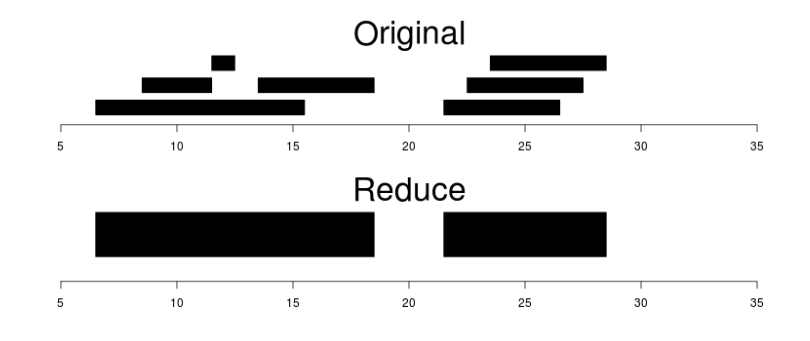
\includegraphics[width=.9\textwidth]{../imgs/reduce.png}
  \end{block}
  \begin{block}{Basic functions}
    \begin{description}
    \item[width] gets the regions size.
    \item[start/end] gets the start/end positions.
    \item[range] gets the range of region (i.e. smallest start + largest end).
    \end{description}
  \end{block}

\end{frame}

\begin{frame}{Exercise - Exon density for one gene}
  \begin{itemize}
  \item Get a \df of the exons for one gene.
  \item Create the corresponding \gr.
  \item Try {\sf width/start/end/range} functions.
  \item ``Reduce'' it.
    \bigskip
  \item Compute the exon density : region covered by exons divided by total region.
  \end{itemize}
\end{frame}

%%%%%
\begin{frame}[fragile, shrink=20]{Apply function on blocks}
  \begin{block}{{\sf do} function}
    \begin{itemize}
    \item Apply a specific function to each block.
    \item Hence input of this function is a \df.
    \item The output as well.
      \bigskip
    \item In the pipe chain {\sf .} represents the input \df.
    \end{itemize}
  \end{block}
  \begin{exampleblock}{Example}
\begin{verbatim}
myDF %>% group_by(colA) %>% head
myDF %>% group_by(colA) %>% do(head(.))

funFunFun <- function(df){
... Instructions on input data.frame 'df'
... creating output data.frame 'new.df'
return(new.df)
}
myDF %>% group_by(colA) %>% do(funFunFun(.))
\end{verbatim}
  \end{exampleblock}
  \begin{alertblock}{Exercise}
    \begin{itemize}
    \item Write a function that computes the exon density from a \df with exons information.
    \item Apply this function to each gene of chromosome 13. 
    \end{itemize}
  \end{alertblock}
\end{frame}

\begin{frame}[fragile]{Parallel processing}
  \begin{block}{Easiest solution with {\sf parallel} package}
    \begin{itemize}
    \item Using \verb!mclapply! instead of \verb!lapply!.
    \item \verb!mc.cores=! the number of processors to use.
    \end{itemize}
  \end{block}
  \begin{exampleblock}{Example}
\begin{verbatim}
lapply(1:10, function(ii){
... Instructions with 'ii'
})

mclapply(1:10, function(ii){
... Instructions with 'ii'
}, mc.cores=4)
\end{verbatim}
  \end{exampleblock}
  \begin{alertblock}{Exercise}
    \begin{itemize}
    \item Compute the exon density of genes in 4 chromosomes, parallelized by chromosome.
    \item Join the output list into one \df using \verb!do.call(rbind, myOutList)!.
    \end{itemize}
  \end{alertblock}
\end{frame}

\begin{frame}[fragile, shrink=10]{Annotation database}
  \begin{block}{Introduction}
    Many annotation are already available directly from R, see Bioconductor website. Else you can create your own {\it GenomicRanges} object.
  \end{block}
  \begin{block}{{\sf AnnotationHub} package}
    Many different tracks, including most of Encode's.
\begin{verbatim}
library(AnnotationHub)
ah = AnnotationHub()
hist.prom = ah$goldenpath.hg19.encodeDCC.wgEncodeBroadHistone.
   wgEncodeBroadHistoneGm12878H3k4me3StdPk.broadPeak_0.0.1.RData
\end{verbatim}      
  \end{block}
  \begin{block}{Exercise}
    \begin{enumerate}
    \item Run these commands.
    \item Have a look at the retrieved object.
    \item How wide is a peak on average ? 
    \item Plot the distribution of the peaks width ?
    \item Remove peaks wider than 10kb.
    \end{enumerate}
  \end{block}
\end{frame}

%%%%%
\begin{frame}[fragile, shrink=10]{Test overlap of one \gr in another}
  \begin{block}{{\sf overlapsAny} function}
    \begin{itemize}
    \item Two {\it GRanges} objects as input.
    \item Returns {\sf TRUE/FALSE} for each range of the first \gr.
    \item {\sf TRUE} means the range overlaps something in the second \gr.
    \item {\sf FALSE} if not.
    \end{itemize}
  \end{block}
  \begin{exampleblock}{Example}
\begin{verbatim}
> any1in2 = overlapsAny(gr1,gr2)
> any1in2
[1]  TRUE  TRUE FALSE FALSE  TRUE FALSE
\end{verbatim}
  \end{exampleblock}
  \begin{alertblock}{Exercise}
    \begin{itemize}
    \item Add a column to the original data.frame with {\sf TRUE/FALSE} if it overlaps a promoter region.
    \item Create some graphs using this new column.
    \end{itemize}
  \end{alertblock}
\end{frame}


\begin{frame}[fragile, shrink=10]{Overlaps between two {\it GRanges} sets}
  \begin{block}{{\sf findOverlaps} function}
    \begin{itemize}
    \item Two {\it GRanges} objects as input.
    \item Extra parameters available for specific overlaps.
    \item Returns the index of regions in object 1 and 2 that overlap.
    \item {\sf queryHits} and {\sf subjectHits} functions to retrieves those index.
    \end{itemize}
  \end{block}
  \begin{exampleblock}{Example}
\begin{verbatim}
> ol12 = findOverlaps(gr1, gr2)
> ol12
Hits of length 3
queryLength: 6
subjectLength: 4
  queryHits subjectHits 
   <integer>   <integer> 
 1         1           1 
 2         2           2 
 3         5           3 
> queryHits(ol12)
[1] 1 2 5
\end{verbatim}
  \end{exampleblock}
  
\end{frame}

\begin{frame}[fragile]{Exercise}
  \begin{enumerate}
  \item Find the overlaps between your genes and the promoters.
  \item Same but allowing +/- 1Kbp for the overlap. See parameter \verb!maxgap=!.
    \bigskip
  \item Create a new \df,  manually merging the promoter {\it score} and your genes annotation \df, for the genes overlapping promoters.
  \item Plot the distribution of the scores for different gene types.
  \end{enumerate}
\end{frame}


\begin{frame}[fragile, shrink=30]{Distance between two {\it GRanges} sets}
  \begin{block}{{\sf distanceToNearest} function}
    \begin{itemize}
    \item Two {\it GRanges} objects as input.
    \item Returns the index of regions in object 1, the closest in 2 and the distance between them.
    \item {\sf queryHits} and {\sf subjectHits} functions to retrieves those index.
    \item {\sf mcols} function to retrieve the distance information.
    \end{itemize}
  \end{block}
  \begin{exampleblock}{Example}
\begin{verbatim}
> d12 = distanceToNearest(gr1, gr2)
> d12
Hits of length 6
queryLength: 6
subjectLength: 4
  queryHits subjectHits  distance 
   <integer>   <integer> <integer> 
 1         1           1         0 
 2         2           2         0 
 3         3           2        10 
 4         4           3         6 
 5         5           3         0 
 6         6           3        21 
> queryHits(d12)
[1] 1 2 3 4 5 6
> mcols(d12)$distance
[1]  0  0 10  6  0 21
\end{verbatim}
  \end{exampleblock}
  
\end{frame}


\begin{frame}{Exercise}
  \begin{enumerate}
  \item Compute the distance between each gene and the nearest promoter.
  \item Add this information as a column in your gene annotation \df.
    \bigskip
  \item Plot the distribution of these distances for different gene types.
  \end{enumerate}
\end{frame}

\begin{frame}[fragile]{More {\it ggplot2} tricks}
  \begin{itemize}
  \item Use \verb!theme(text=element_text(size=22))!.
  \item Use \verb!scale_fill_brewer(palette="Set1")!.
  \item Use \verb!scale_x_discrete(limits=)!.
  \end{itemize}
\end{frame}

\begin{frame}[fragile]{Boxplots}
  \begin{block}{}
    \begin{itemize}
    \item \verb!geom_boxplot! function.
    \item \verb!x=! to define the x-coordinate.
    \item \verb!y=! to define the y-coordinate.
      \bigskip
    \item \verb!fill=! to define the box color.
    \item Optional: \verb!group=! to define what's in the box.
    \end{itemize}
  \end{block}
  \begin{exampleblock}{Example}
\begin{verbatim}
ggplot(myDF,aes(x=colA, y=colB)) + geom_boxplot()

ggplot(myDF,aes(x=colA,y=colB,fill=colC)) + geom_boxplot()

ggplot(myDF,aes(x=colA,y=colB,group=colC)) + geom_boxplot()
\end{verbatim}
  \end{exampleblock}
  \begin{alertblock}{Exercise}
    Make some boxplots, maybe using the gene expression \df.
  \end{alertblock}
\end{frame}


\begin{frame}[shrink=15]{Online resources}
  \begin{block}{R basics}
    \begin{itemize}
    \item \url{http://www.twotorials.com/} : small video-tutorials.
    \item \url{www.youtube.com/user/rdpeng/} : Coursera {\it Computing for Data Analysis} videos. Other interesting videos, e.g. {\it ggplot2}.
      \bigskip
    \item \url{https://www.datacamp.com/} or \url{http://tryr.codeschool.com/} : Interactive tutorial of R basics.
      \bigskip
    \item \url{http://www.r-tutor.com/} : R and statistics small web-tutorials.
    \item \url{http://www.computerworld.com/s/article/9239625/Beginner_s_guide_to_R_Introduction} : Beginner's guide with screenshots.      
    \item \url{http://cran.r-project.org/manuals.html} : R manual.
    \end{itemize}
  \end{block}
  
  \begin{block}{Bioinformatics}
    \begin{itemize}
    \item \url{http://stephenturner.us/p/edu} List of online resources for Bioinformatics.
    \item \url{http://bioinformatics.ca/workshops/2013/} : Bioinformatics workshop material.
    \item \url{http://manuals.bioinformatics.ucr.edu/home/R_BioCondManual} : Pieces of code for bioinformatics analysis, plots. Including Bioconductor.
    \item \url{http://bioconductor.org/help/course-materials/2013/} : Bioinformatics tutorials material: pdf and R scripts.
    \end{itemize}
  \end{block}


\end{frame}


%% TODO Exercises with GRanges
%% GGPLOT2 tricks : text size; aes and different datasets, density, colors

\end{document}

